Prvi korak u analizi argumentacije je prepoznavanje, strukturiranje i 
izrada argumenata iz argumentativne rasprave \citep{scheuer2010computer,
prudencio2005visualizing}. Izrada argumenata iz teksta
radi se izdvajajući tekst koji odgovara
specifičnim dijelovima argumenata, 
povezujući dijelove argumenta ih odgovarajućim relacijama. 
Tako u tekstu \emph{Student
Ivo polaže PZUIS;\ Student Ivo mora samo položiti PZUIS prije nego doktorira;\ Student
Ivo može doktorirati} možemo izdvojiti \textbf{premise} \emph{Student
Ivo polaže PZUIS;\ 
} i 
\emph{Student
Ivo mora položiti PZUIS prije nego doktorira
} te \textbf{zaključak}
\emph{Student Ivo može doktorirati} te izvesti da
iz premisa slijedi zaključak modus ponens pravilom zaključivanja. 
Analiza uključuje 
proučavanje valjanosti zaključivanja te
kvalitete premisa i zaključka.

Razvojem softvera za argumentaciju, 
olakšala se i analiza argumentacije. \textbf{Araucaria}
je najpopularniji softver za analizu argumentaciju s 10000 korisnika iz
preko 80 zemalja između 2001.\ i 2010.\ 
godine~\citep{Chris2017-REETAW}. Araucariom se mogu
\begin{enumerate}
\item izrađivati dijagrami argumenata iz tekstnih datoteka,
\item uređivati korištene argumentacijske modele i 
\item pohranjivati argumente (više u poglavlju~\ref{chap:aif})
\end{enumerate}
Omogućavanjem uređivanja argumentacijskih modela, Arauciaria
je prvi alat agnostičan na model argumentacije
pretpostavljajući Toulminov model argumenta, ali zadržavajući kompatibilnost
s Wigmoreovim \citep{wigmore2016wigmore} i 
Freemanovim \citep{freeman1991dialectics} modelima. 
Zbog svoje kompatibilnosti s više različitih argumentacijskih 
modela, Araucia se smatra realizacijskim začetnikom argument weba.
Araucaria je 
danas\footnote{7.1.2018.\ dostupna na URL-u \url{http://ova.arg-tech.org/}} 
dostupna online pod imenom OVA \engl{Online Visualization of Argument}. 

\section{Kolaborativna analiza}

\begin{figure}
\centering
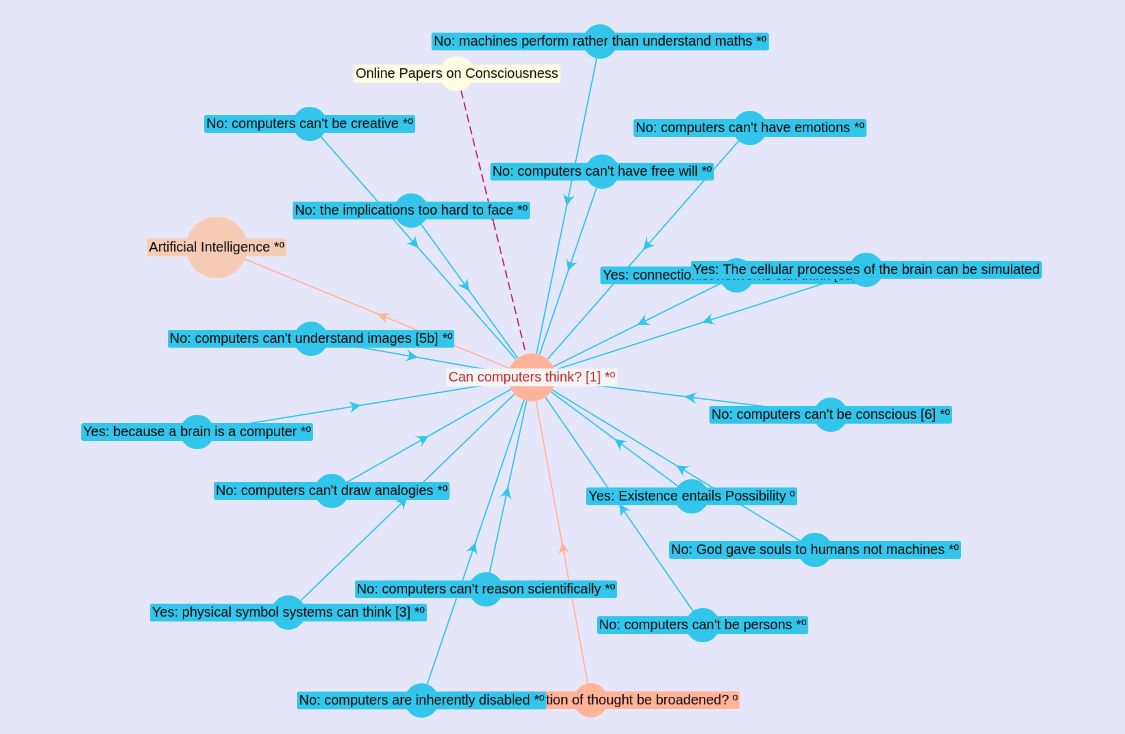
\includegraphics[scale=0.4]{debategraph.png}
\caption{Analiza mogu li računala razmišljati na DebateGraphu}
\label{fig:computers}
\end{figure}

Postavljanje sustava za analizu argumenata online olakšalo je suradnju 
na analizi argumentacije koja je neophodna u slučaju kompleksnije
argumentacije. Uz OVA alat, pojavili su se i drugi online alati za
analizu argumentacije. DebateGraph\footnote{7.1.2018.\ dostupno na 
\url{https://www.debategraph.com}} omogućava korisnicima hijerarhijsku 
analizu teme kroz grafove. Primjer na slici~\ref{fig:computers} prikazuje
analizu \emph{Mogu li računala razmišljati} u sustavu DebateGraph. Svaki
čvor u grafu moguće je dodatno otvoriti i zasebno istražiti. 

\begin{figure}
\centering
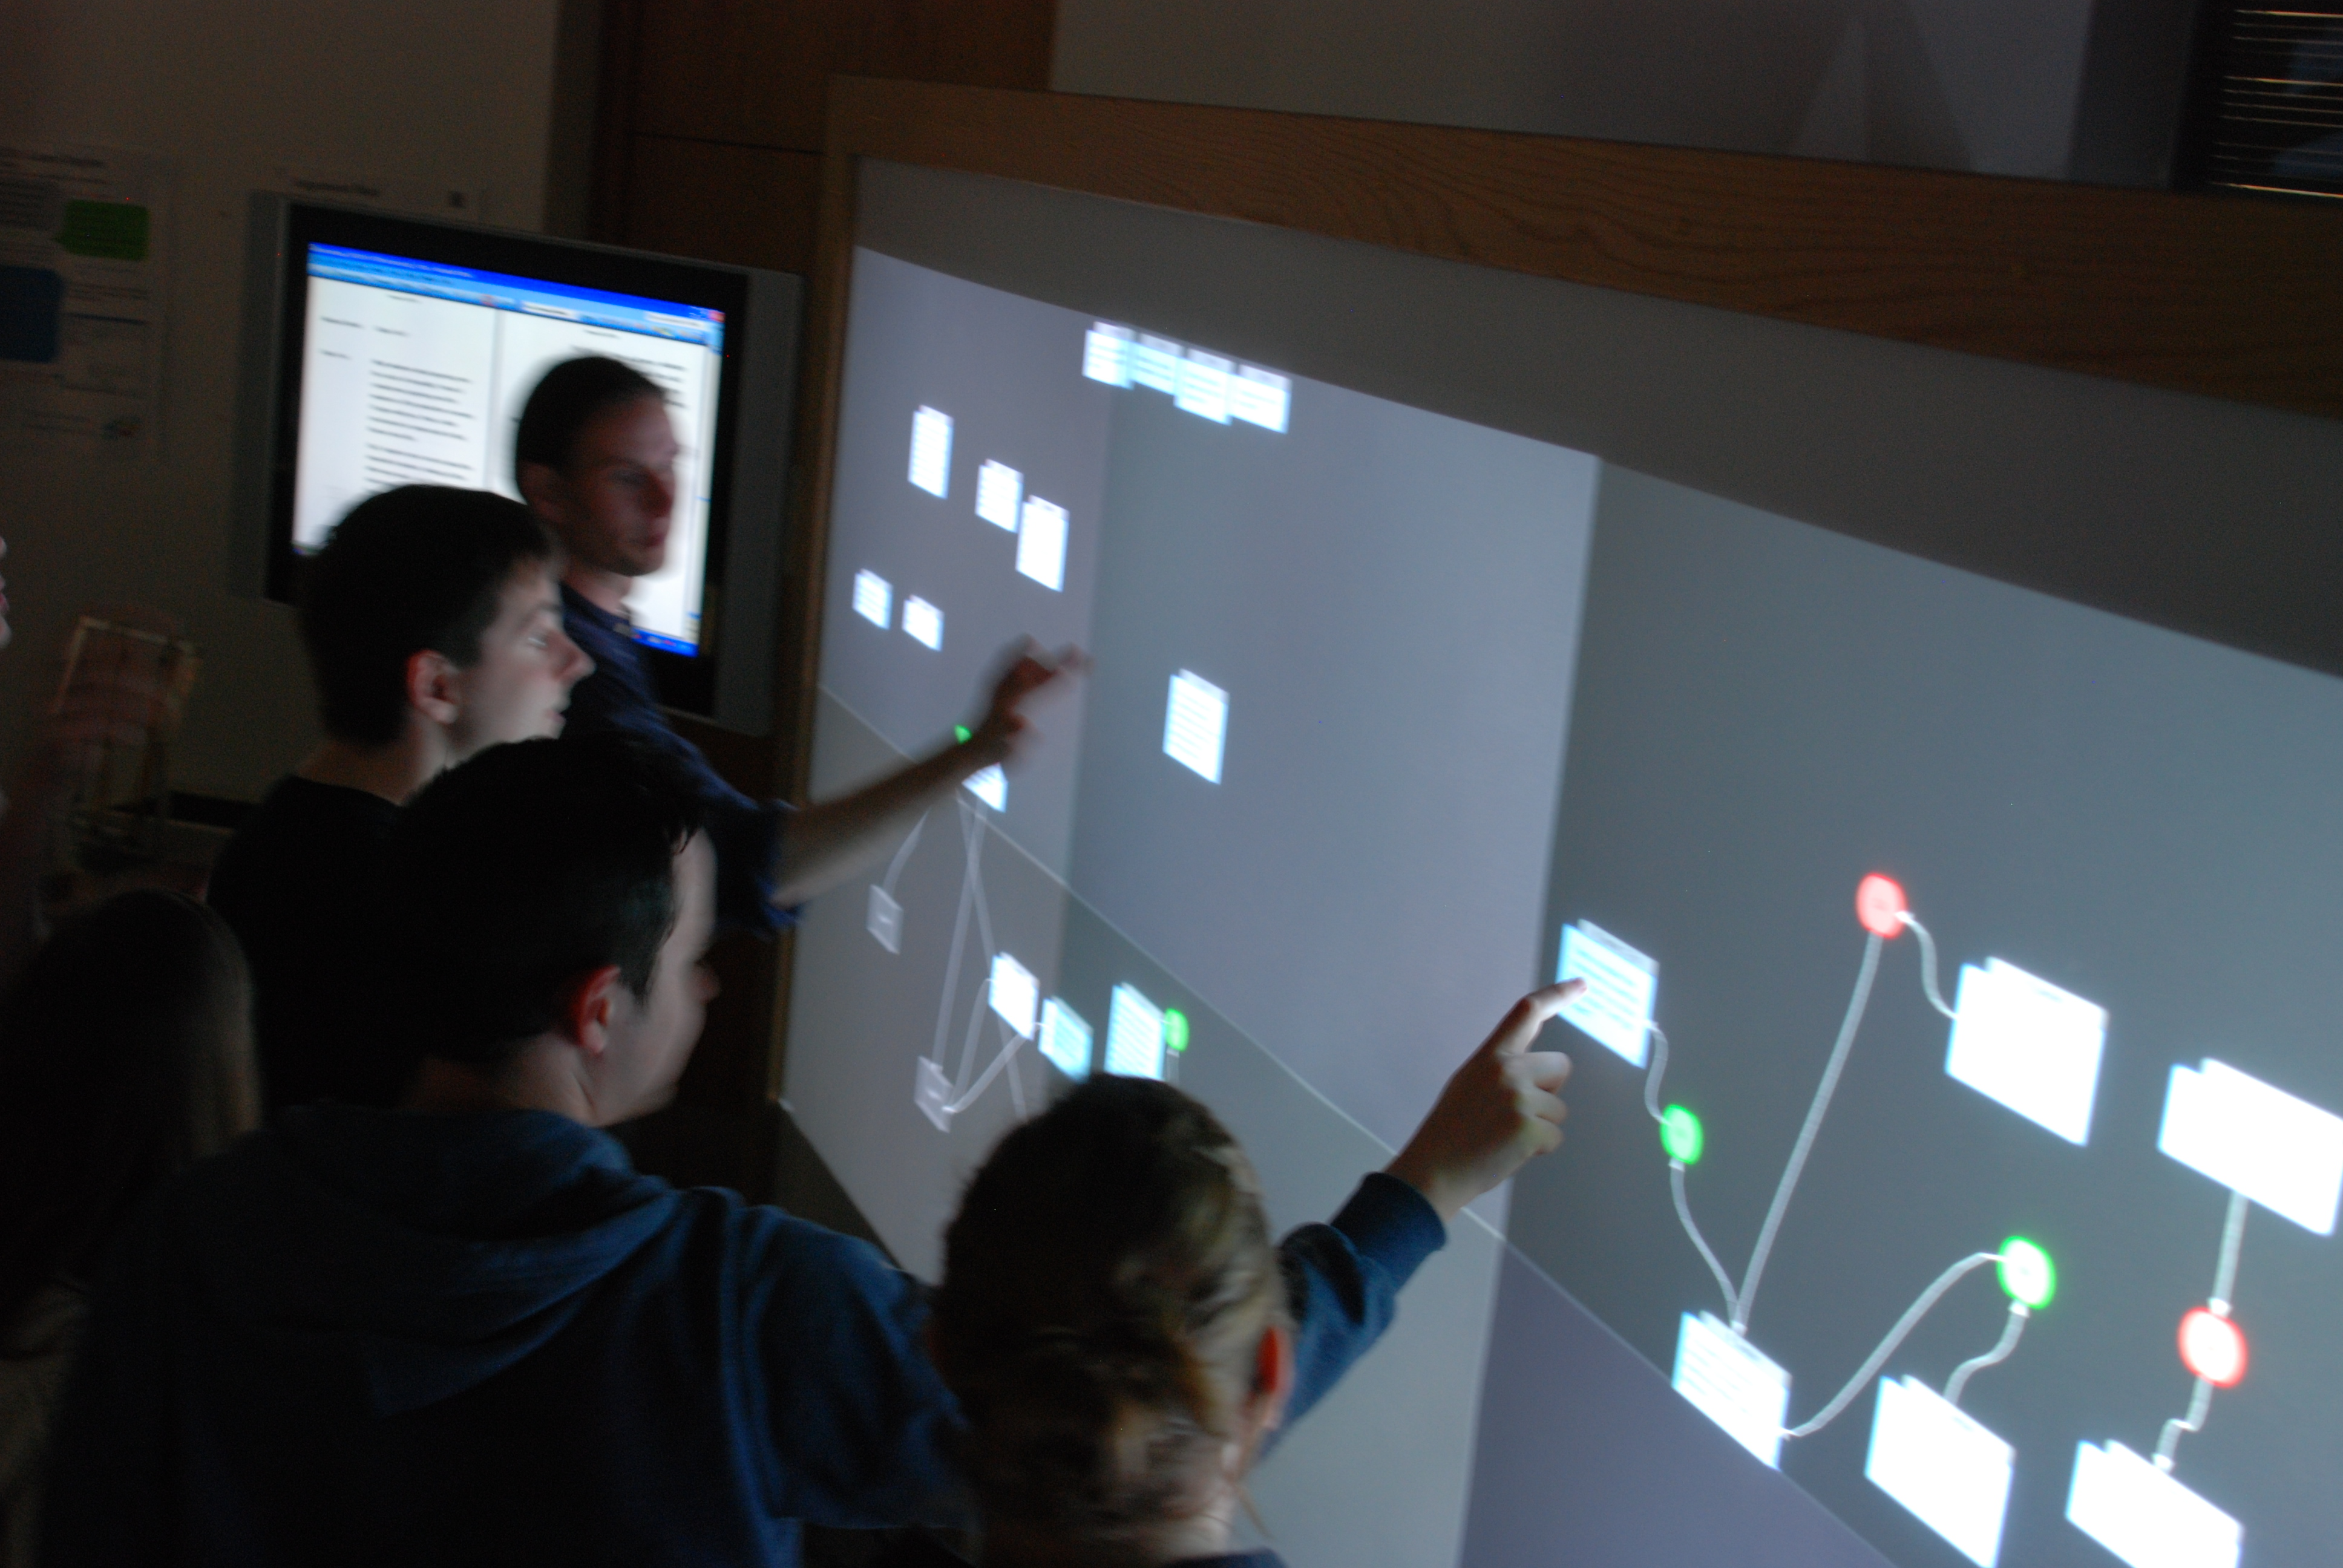
\includegraphics[scale=0.4]{analysis_wall.jpg}
\caption{Anotacija pomoću AnalysisWall-a}
\label{fig:analysiswall}
\end{figure}

Kolaborativna analiza argumentacije u stvarnom vremenu moguća je uz alat 
škotske grupe znanstvenika
AnalysisWall\footnote{7.1.2018.\ više o projektu na \url{http://www.arg-tech.org/index.php/projects/argument-analysis-wall/}}.
Uz AnalysisWall moguće je analizirati debatu, prepoznavati i povezivati argumente 
koristeći video zaslon na dodir, kao što je učinjeno na slici~\ref{fig:analysiswall}.
